\chapter{Usability Experiment}\label{ch:experiment}
This chapter will present the design and execution of an experiment trying to measure  the performance of the human computable password management scheme. The experiment is design as a web application implementing the scheme allowing participants to test how the scheme would work in practice while measuring how fast the computation is performed. The application thus acts as both a demonstration app and a tool for gathering performance data. It has four sections designed to help the participants understand the scheme and get familiar with the computation technique. First as demonstration video is displayed explaining how to compute a password from a challenge, then the user is asked to enter some demographic data. Next is the practice section, where the user is supposed to practice doing the calculation until being able to solve challenges without error. Finally is the experiment part, which is timed and correctness monitored. After finishing the calculations the user will submit the data and can chose to continue doing more experiments. 
\section{Experiment Objective.}
\todo[inline]{Explain what the goal of the experiment is. What results I'm looking for/what the purpose is.}
\todo[inline]{NOTE: The experiment application is not only recording data, it works as a presentation of the scheme, trying to make it easy to understand so that most people should be able to use it. }
The goal of the experiment is to measure how hard it is for a user to learn the scheme, and namely how fast users do the calculations. The experiment will thus measure the calculation times of different users, and also monitor their progress after several trials. Hopefully a user will be able to calculate passwords without to many mistakes. The failure rate is maybe the most important variable to measure; if a user average more than one mistake for each password calculated the scheme would not work in practice, since most passwords calculated would be wrong. 
\par It is important to note that this project does not see the human computable password management scheme as a replacement for the widen used standard password managers. It is regarded as a solution for users interested in a secure and reliable way of keeping track of strong password, without having to trust a password management service or application. This experiment will thus test if it is even possible, for a user willing to go through the trouble of learning a secret mapping, to use the scheme as an everyday solution.

\par The objectives of the experiment can be summarized as the following.
\begin{itemize}
    \item Measure the average calculation times, both for each participants and for the whole population.
    \item Measure how much the users improve after several trials.
    \item Measure the average failure rate for each participant.
\end{itemize}


\subsection{Method}
The experiment does not try to test any preset hypothesis as it is not clear what to expect regarding either of the tested values. It is not known how hard it is to to the calculations, neither regarding calculation time or failure rates. The results of the experiment will not be a clear answer to any hypothesis, but rather a basis for further data collection through larger scale experiments, in example using crowd sourcing or social medias.

\par Exploratory data analysis (EDA) was introduced by John W. Turkey~\cite{turkey} which involves analysis of data without a prior hypothesis to test. The technique promotes exploration of data to possible find characteristics not previously considered, and essentially suggesting hypotheses to be tested later surveys or experiments. Velleman and Hoaglin~\cite{exploratory-analysis} describes EDA as a contrast to the formal scientific method involving stating a hypothesis, collecting data and applying a statistical test of the hypothesis. EDA often involves making graphical representations of the data, and then try to find interesting characteristics and relations. EDA does not conclude with a hypothesis test based on the collected data, but is the first step of an iterative process trying to reveal facts. 
\par This project does not intend to test any hypothesis, but rather gather data thought to be relevant, in this case, calculation time and failures, then display the data as graph and investigate relationships between different statistics. The findings of the experiment should be seen only as a prerequisite for later experiments, the patterns found can be used to form a more specific statistical test.
\par The project will not store any personal information about the participants, and should thus not be subject to notification to the "Norwegian Social Science Data Service"\footnote{Is my research project subject to notification? - \url{http://www.nsd.uib.no/nsd/english/pvo.html}}. The experiment will only record an anonymous id plus the experiment results consisting of computation time and correctness of the calculations done. Some demographic data will also be recorded (age, area of study), but the data can not be connected to person and are thus not regarded as personal information.

\par After conducting the experiment, the data will be examined and significant characteristics discussed. There are some obvious parameters to explore, including means and standard deviation of the calculation times and failure rate, as well as how these change with practice. 

\par The usability of the scheme directly rely on the calculation time and failure rate as discussed in section \ref{sec:usability}. This can be discussed further after obtaining some numbers giving a picture of what is normal and possible in terms of speed and reliability.
\par A result showing that more than 90\% of all calculations are correct would be promising, since it means that more than 50\% of the passwords calculated would actually be correct. If this is not the case the scheme would more often than not be useless since most users would obtain a faulty password when trying to log in. The conclusion of the experiment presented in this project, will either way have to be tested more thorough, possibly using the same experiment setup or preferably with a throughly random mapping as well. 



\section{Experiment Setup}
\todo[inline]{What data will be recorded, choices regarding the secret mapping etc.}
The experiment will present and demonstrate the calculation technique to the user, which then will be given a chance to practice until fairly familiar with the mechanics. Finally the user will be asked to calculate a complete password challenge, from which the time spent on each single digit challenge will be recorded, as well as if the calculation was correct or not. The practice section will allow the user to try and fail, using backspace to go back and forth between challenges while also giving feedback on the correctness. The experiment view on the other hand will not give any feedback and does not allow the user to go back after entering a character. This is done to make sure all mistakes are recorded, even if it is only a miss click. 
\subsection{Secret mapping} The biggest decision made in regards to the experiment design was how to simulate "recalling" from memory. It would not be feasible to ask all the participants to memorize a secret mapping on beforehand as this would probably make it impossible to find volunteers. The chosen solution to this problem is to include a "cheat sheet" in addition to the displayed challenges, this will be a list of object to digit mappings shown separately but in the same view as the challenge.
\par After some testing it became apparent that the there was a big difference between recalling from memory and actually "reading" from a list, which this approach eventually is. To make the operation more similar to the desired recall operation, the mapping was changed from random to mirror the alphabet with accompanying position(e.g A=1, B=2, C=3). This way one does not have to read in the table to know correct mapping for all letters at least. Most users will be able to know instantly what the mapping for at least the first and eventually, after some practice, all the letters. The is the closest way of mimicking the actual operations of the scheme without having the participants memorize an actual mapping. It is not in any way certain that this shortcut reflect the real world act of recalling from memory, but it is assumed to be "close enough" for the experiment. The author of this project did memorize a mapping of both 10 and later 20 mappings without significantly different calculation times compared to using the alphabet positions.


\subsection{Participants}
The participants for the experiment was chosen mostly from people known by the author, this limits the number of participants somewhat. This was done to ensure the quality of the data samples. The experiment could have been distributed through crowd sourcing services or social media, probably increasing the number of participants drastically. The problem with this approach, and the reason for not doing it, is that the experiment requires absolute concentration which can not be assured from "casual" participants accessing the experiment through a link posted on facebook. 
\par The results from the experiment is thus restricted  by the limit number of participants, but the results are still considered to be interesting. Since the scheme tested is not supposed to be a widely-deployed password manager, it might be sufficient if the experiment can show that some users are able achieve what is considered sufficient usability. 




\subsection{Web Application}
\todo[inline]{Design and architecture of the web application}
\todo[inline]{Discuss if a similar application could be used as an actual password manager. What are the advantages/disadvantages versus the extension implementation. }
The experiment application will be similar in design to the Chrome extension presented in \autoref{app}, but implemented as a web application. The application will consist of four sections to flip through, with the last one being the actual experiment.  First the user will be presented with a presentation of the scheme and how to calculate passwords, this will be in the form of a demo presentation with instructions. The slides used to instruct the user can be seen in \autoref{demo-slides}, these will be parts of a video in the first view of the web application. After watching the video, the user if asked to enter some demographic data (age and occupation). Next, is a section which looks the same as the experiment, but without the actual recording of data, this is the practice section. The purpose of this section is to give the user a chance to verify that he has understood the scheme and are actually able to calculate passwords. When the user is ready to start the experiment, he can continue on to the actual experiment, which is the final view. 

\par The experiment is exactly like the practice section, without response on correctness and redo capabilities, with backspace deactivated. The first sample of the experiment will not be counted towards the results, to allow the user to get ready and start when he feels like it. 
\par Section \ref{computation-time} discussed how a single digit challenge can be presented to the user in a logical way, possibly making it more efficient to calculate. The experiment use a similar layout to the one shown in \autoref{challenges} and also as in the Chrome extension in Chapter \ref{app}. The challenges will update in the same way as in the chrome extension so the user should be able to calculate the responses continuously. The calculation time is recorded for each challenge computed, together with a boolean value representing if the result was correct or not. 
\par Figure \ref{complete-experiment} shows the screen after completing a trail of the experiment, next the user would push the submit button and the sample would be saved in the database together with a random identification stored in a cookie in the user's browser. The user can then redo the experiment several times keeping the same id, making it possible to track each participant's development.

\begin{figure}[h]
    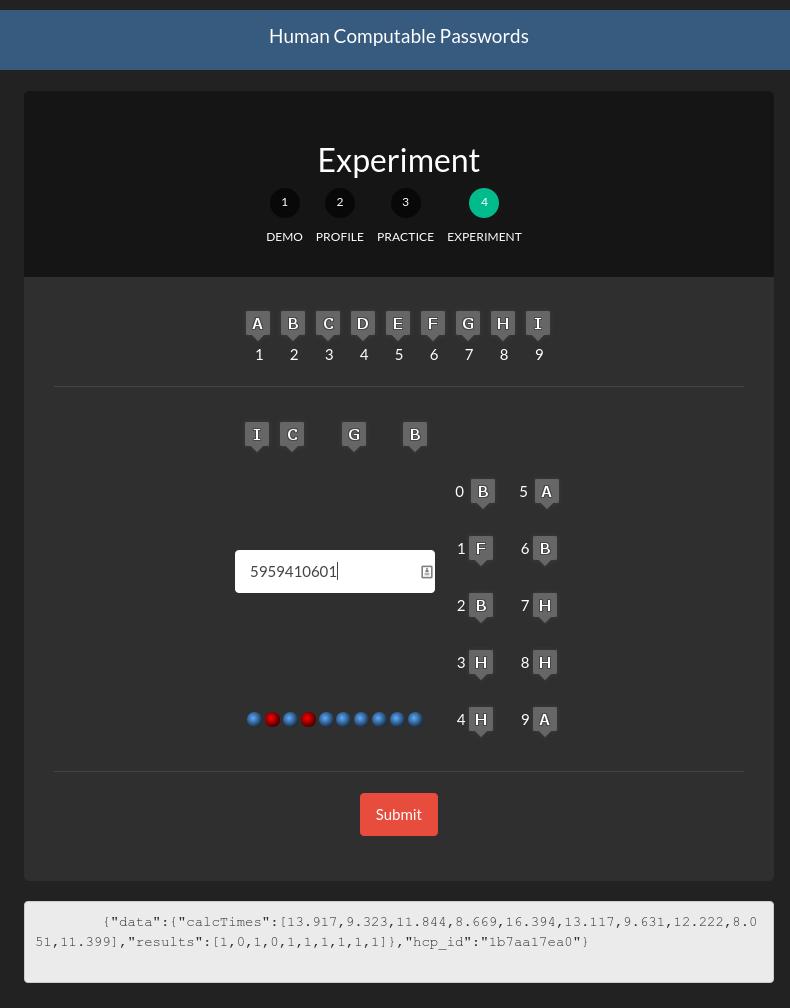
\includegraphics[width=\textwidth]{complete-experiment}
    \caption{The experiment screen seen after completing an experiment sample, ready to be submitted.}
    \label{complete-experiment}
\end{figure}

\par The views of the web application can be seen in \autoref{experiment-views} or by visiting the hosted experiment site at \url{hcp.sp1nakr.com}.


\subsection{Results}
\todo[inline]{Presentation of the results gather through the experiment (calculation time, failure rate etc. )}
\todo[inline]{Different plots of the data. Not sure what and how to plot the different data??}


\begin{figure}
    \centering
    \begin{tikzpicture}
        \begin{axis}[width=\textwidth, xlabel=Calculation times in seconds. ,ybar, ymin=0, yticklabels={,,}]
            \addplot +[
                    hist = {
                        bins=20,
                        data min=3,
                        data max=20
                    },
                    fill=blue!60
                ]table [y index=0]{calcTimes.csv};

        \end{axis}
    \end{tikzpicture}
    \caption{Histogram showing the distribution of calculation times of all the recorded experiments. Sample size $342$ single digit challenges.}
    \label{histo-calctimes}
\end{figure}

\begin{figure}
    \centering
\begin{tikzpicture}
    \begin{axis}[
                enlargelimits=false,
                xlabel=Trial number: $i$,
                ylabel = Average calculation time in seconds.,
                width=\textwidth,
                ymin=4,
                ymax=18
        ]
        \addplot+[
                only marks,
                scatter,
                mark size=1.5pt
            ]
            table[meta=avg]
            {sum-avgs.dat};
        \addplot[
            domain=0:80,
            samples=3,
            very thick
        ]{12.56074424-0.06942622*x};
    \end{axis}

\end{tikzpicture}
\caption{Average calculation time of all participants' $i'th$ calculation sample, and the regression line of the averages. Sample size $342$, average samples per participant $31$.}
\label{scatter-regression}
\end{figure}




\subsection{Discussion}
\todo[inline]{Discuss how the results fit in the usability model, plots $\hat t$ for the different participants}
\todo[inline]{What use cases would require a faster or slower calculation time?}
\todo[inline]{}
